
\chapter{Delayed Simulation}
\label{chap:fritzwilke}

\section{Theory}

In this part we consider delayed simulation and variants thereof on DPAs. This approach is based on the paper \cite{FritzWilke06}, which considered the games for alternating parity automata. The DPAs we use are a special case of these APAs and therefore worth examining.

\begin{defn}
	Let $\mathcal{A} = (Q_1, \Sigma, \delta_1, c_1)$ and $\mathcal{B} = (Q_2, \Sigma, \delta_2, c_2)$ be DPAs. For $\alpha \in \Sigma^\omega$, we write $(\mathcal{A}, p) \leq_\text{de}^\alpha (\mathcal{B}, q)$ iff the following holds:
	
	Let $\pi$ and $\rho$ be the runs of $\mathcal{A}$ and $\mathcal{B}$ on $\alpha$ starting in $p$ and $q$ respectively. For every position $i$, there is a $j \geq i$ such that $\pi(i) \leq \min \{c_1(p'), c_2(q')\}$ is odd or $\rho(i) \leq \min \{c_1(p'), c_2(q')\}$ is even, where $p' = \pi(i)$ and $q' = \rho(i)$.
	
	We define \emph{delayed simulation} as $(\mathcal{A}, p) \leq_\text{de} (\mathcal{B}, q)$ iff $(\mathcal{A}, p) \leq_\text{de}^\alpha (\mathcal{B}, q)$ is true for every $\alpha$.
\end{defn}

This definition might seem arbitrary. It is adapted to the result of delayed simulation games from \cite{FritzWilke06} that we describe later on. A more intuitive descendant of $\leq_\text{de}$ is delayed simulation equivalence $\equiv_\text{de}$ that is defined below.

\begin{defn}
	We define $(\mathcal{A}, p) \equiv_\text{de} (\mathcal{B}, q)$ iff both $(\mathcal{A}, p) \leq_\text{de} (\mathcal{B}, q)$ and $(\mathcal{B}, q) \leq_\text{de} (\mathcal{A}, p)$.
\end{defn}

\begin{lem}
	\label{lem:fritzwilke:equivde_alternative}
	$(\mathcal{A}, p) \equiv_\text{de} (\mathcal{B}, q)$ if and only if the following property holds for all $w \in \Sigma^*$: 
	
	Let $p' = \delta_1^*(p, w)$ and $q' = \delta_2^*(q, w)$. Every run that starts in $p'$ or $q'$ eventually sees a priority less than or equal to $\min \{c_1(p'), c_2(q')\}$.
\end{lem}

\begin{proof}
	\textbf{If } We show that $(\mathcal{A}, p) \leq_\text{de} (\mathcal{B}, q)$. The other inclusion follows by symmetry. Let $\alpha \in \Sigma^\omega$ and let $\pi$ and $\rho$ be the runs on $\alpha$ starting in $p$ and $q$. Let $i$ be a position, $p' = \pi(i)$, and $q' = \rho(i)$. Assume that there is no $j \geq i$ such that $\pi(j)$ is odd and $c_1(\pi(j)) \leq \min \{c_1(p'), c_2(q')\}$. We will show that there must be a $j \geq i$ where $c_2(\rho(j)) \leq \min \{c_1(p'), c_2(q')\}$ is even.
	
	By assumption of the Lemma, there is a $j$ with $\rho(j) \leq \min \{c_1(p'), c_2(q')\}$. If any of these $j$ is even, we are done; otherwise, they are all odd. Let $j$ be chosen such that $\rho(j)$ is minimal. There must be a $k \geq j$ such that $c_1(\pi(k)) \leq \min \{c_1(\pi(j)), c_2(\rho(j))\}$. This value cannot be odd, as $c_1(\pi(k)) \leq c_2(\rho(j)) \leq \min \{c_1(p'), c_2(q')\}$ happens only at even values. Hence, it must also be strictly smaller than $c_2(\rho(j))$.
	
	We can apply the assumption one last time, to find a position $l \geq k$ such that $c_2(\rho(l)) \leq \min \{c_1(\pi(k)), c_2(\rho(k))\} < c_2(\rho(j))$ which contradicts the choice of $j$ to have minimal priority.
	
	\paragraph{Only If } Assume $(\mathcal{A}, p) \equiv_\text{de} (\mathcal{B}, q)$. We show that the described property is true. Towards a contradiction, assume that there are $w$ and $\beta$ such that from $p'$ and $q'$ one of the runs $\pi$ and $\rho$ only visits priorities greater than $\min \{c_1(p'), c_2(q')\}$. Without loss of generality, let that run be $\pi$.
	
	Let $i > |w|$ be a position such that $c_2(\rho(i))$ becomes minimal. If that value is odd, consider $(\mathcal{A}, p) \leq_\text{de} (\mathcal{B}, q)$; there must be a position $j \geq i$, such that $c_1(\pi(j)) \leq \min \{c_1(\pi(i)), c_2(\rho(i))\}$ is odd or $c_2(\rho(j)) \leq \min \{c_1(\pi(i)), c_2(\rho(i))\}$ is even. The first case cannot happen, as then $\pi$ would visit a priority less than $\min \{c_1(p'), c_2(q')\}$. The second case however cannot be true either, as $c_2(\rho(i))$ is odd and there is no priority in $c_2(\rho)$ smaller than that value. 
	
	If $c_2(\rho(i))$ would be even, we could use $(\mathcal{B}, q) \leq_\text{de} (\mathcal{A}, p)$ to find a similar contradiction.
\end{proof}

\begin{lem}
	$\equiv_\text{de}$ is a congruence relation.
\end{lem}

\begin{proof}
	Using the characterization of $\equiv_\text{de}$ in Lemma \ref{lem:fritzwilke:equivde_alternative} easily shows that it is an equivalence relation.
	
	Now to show that $\equiv_\text{de}$ is also a congruence relation: Let $(\mathcal{A}, p) \equiv_\text{de} (\mathcal{B}, q)$ and $a \in \Sigma$. We want to prove that also $(\mathcal{A}, p') \equiv_\text{de} (\mathcal{B}, q')$ with $p' = \delta_1(p, a)$ and $q' = \delta_2(q, a)$. Assume that this is not the case, so there is a $w \in \Sigma^*$ such that the following is true for $p'' = \delta^*_1(p', w)$ and $q'' = \delta^*_2(q', w)$: $c_1(p'') < c_2(q'')$ and there is a run starting in $q''$ that only sees priorities greater than $c_1(p'')$. Then, however, we could also reach $p''$ and $q''$ from $p$ and $q$ by the word $aw$ which implies that $(\mathcal{A}, p) \not\equiv_\text{de} (\mathcal{B}, q)$.
\end{proof}

\vspace{15pt}

We move on to establishing $\equiv_\text{de}$ as a \enquote{good} relation for our needs and define a fitting merger function.

\begin{lem}
\label{lem:fritzwilke:equiv_states_same_minpri}
	Let $\mathcal{A}$ be a DPA and let $\pi$ and $\rho$ be runs of $\mathcal{A}$ on the same word $\alpha$ but starting at different states. If $\pi(0) \equiv_\text{de} \rho(0)$, then $\min \text{Occ}(c(\pi)) = \min \text{Occ}(c(\rho))$.
\end{lem}

\begin{proof}
	Let $\pi(0) = p$ and $\rho(0) = q$. Assume towards a contradiction that the statement is false and $\min \text{Occ}(c(\pi)) < \min \text{Occ}(c(\rho))$. Let $k = \min \text{Occ}(c(\pi))$ and let $n$ be the first position at which $c(\pi(n)) = k$. Let $p' = \pi(n)$ and $q' = \rho(n)$. These two states are reachable from $p$ and $q$ respectively with the word $\alpha[0,n]$.
	
	By Lemma \ref{lem:fritzwilke:equivde_alternative}, the run $\rho[n,\omega]$ must eventually see a priority at most $k$ which contradicts the assumption.
\end{proof}


\begin{theorem} 
\label{thm:fritzwilke:combine_priorities}
	Let $\mathcal{A} = (Q, \Sigma, \delta, c)$ be a DPA and let $p, q \in Q$ with $p \equiv_\text{de} q$ and $c(p) < c(q)$. Define $\mathcal{A}' = (Q, \Sigma, \delta, c')$ with $c'(s) = \begin{cases} c(p) & \text{if } s = q \\ c(s) & \text{else} \end{cases}$. Then $\mathcal{A} \equiv_L \mathcal{A}'$.
\end{theorem}

\begin{proof}
	Let $q_0 \in Q$ be an arbitrary state. We show that $L(\mathcal{A}, q_0) = L(\mathcal{A}', q_0)$.
	
	First, consider the case that $c(p)$ is an even number. The parity of each state is at least as good in $\mathcal{A}'$ as it is in $\mathcal{A}$, so $L(\mathcal{A}, q_0) \subseteq L(\mathcal{A}', q_0)$. For the other direction, assume there is an $\alpha \in L(\mathcal{A}', q_0) \setminus L(\mathcal{A}, q_0)$, so the respective run $\rho \in Q^\omega$ is accepting in $\mathcal{A}'$ but not in $\mathcal{A}$. 
	
	For this to be true, $\rho$ must visit $q$ infinitely often and $c'(q)$ must be the lowest priority that occurs infinitely often; otherwise, the run would have the same acceptance in both automata. Thus, there is a finite word $w \in \Sigma^*$ such that from $q$, $\mathcal{A}$ reaches again $q$ via $w$ and inbetween only priorities greater than $c'(q)$ are seen.
	
	Now consider the word $w^\omega$ and the run $\pi_q$ of $\mathcal{A}$ on said word starting in $q$. With the argument above, we know that the minimal priority occuring in $c(\pi_q)$ is greater than $c'(q)$. If we take the run $\pi_p$ on $w^\omega$ starting at $p$ though, we find that this run sees priority $c(p) = c'(q)$ at the very beginning. This contradicts Lemma \ref{lem:fritzwilke:equiv_states_same_minpri}, as $p \equiv_\text{de} q$. Thus, the described $\alpha$ cannot exist. 
	
	If $c(p)$ is an odd number, a very similar argumentation can be applied with the roles of $\mathcal{A}$ and $\mathcal{A}'$ reversed. We omit this repetition.
\end{proof}

\vspace{5pt}

Together with Lemma \ref{lem:general:congrel_prio_implies_moore}, this allows for a merger function that preservers language.

\begin{defn}
	We define the \emph{delayed simulation merger} as $\mu_\text{de} : \mathfrak{C}(\equiv_\text{de}) \rightarrow 2^Q$ with $\mu_\text{de}(\kappa) = \{ q \in \kappa \mid c(q) = \min c(\kappa) \}$.
\end{defn}

\begin{cor}
	Let $\mathcal{A}$ be a DPA. Then $\mathcal{A}$ is language equivalent to every representative merge w.r.t. $\mu_\text{de}$.
\end{cor}

\begin{proof}
	With Theorem \ref{thm:fritzwilke:combine_priorities}, we can construct a language equivalent $\mathcal{A}' = (Q, \Sigma, \delta, c')$ such that for all $\kappa \in \mathfrak{C}(\equiv_\text{de})$, all states in $\kappa$ have the same priority in $c'$. Every representative merge of $\mathcal{A}$ w.r.t. $\mu_\text{de}$ is a representative merge of $\mathcal{A}'$ w.r.t. $\mu_\text{de}$.
	
	In $\mathcal{A}'$, $\mu_\text{de}$ is the same as $\mu^{\equiv_\text{de}}_\div$. The fact that representative merges of $\mathcal{A}'$ w.r.t. $\mu_\text{de}$ preserve language follows from Lemma \ref{lem:general:congrel_prio_implies_moore}.
\end{proof}



\section{Computation}
So far we have given a definition of $\equiv_\text{de}$ that provides no obvious way of how to compute that relation. For that we can use delayed simulation games as described in \cite{FritzWilke06}.

\begin{defn}
	We introduce $\checkmark$ as an \enquote{infinity} to the natural numbers and define the \textbf{obligation order} $\leq_\checkmark \subseteq (\mathbb{N} \cup \{\checkmark\}) \times (\mathbb{N} \cup \{\checkmark\})$ as $0 \leq_\checkmark 1 \leq_\checkmark 2 \leq_\checkmark \dots \leq_\checkmark \checkmark$.
	
	Second, we define an order of \enquote{goodness} on parity priorities $\preceq_\text{p} \subseteq \mathbb{N} \times \mathbb{N}$ as $0 \preceq_\text{p} 2 \preceq_\text{p} 4 \preceq_\text{p} \dots \preceq_\text{p} 5 \preceq_\text{p} 3 \preceq_\text{p} 1$.
\end{defn}

\begin{defn}
	Let $\mathcal{A} = (Q_1, \Sigma, \delta_1, c_1)$ and $\mathcal{B} = (Q_2, \Sigma, \delta_2, c_2)$ be DPAs. We define the \emph{delayed simulation automaton} $(\mathcal{A},\mathcal{B})_\text{de} = (Q_\text{de}, \Sigma, \delta_\text{de}, F_\text{de})$, which is a deterministic Büchi automaton, as follows.
	
	\begin{itemize}
		\item $Q_\text{de} = Q_1 \times Q_2 \times (c_1(Q_1) \cup c_2(Q_2) \cup \{ \checkmark \})$, i.e. the states are given as triples in which the first two components are states from $\mathcal{A}$ and the third component is either a priority from $\mathcal{A}$ or $\mathcal{B}$ or $\checkmark$.
		\item The alphabet remains $\Sigma$.
		\item $\delta_\text{de}( (p, q, k), a ) = ( p', q', \gamma(c_1(p'), c_2(q'), k)$, where $p' = \delta_1(p, a)$, $q' = \delta_2(q, a)$, and $\gamma$ is the same function as used in the initial state. The first two components behave like a regular product automaton.
		\item $F_\text{de} = Q_1 \times Q_2 \times \{ \checkmark \}$.
	\end{itemize}
	
	$\gamma : \mathbb{N} \times \mathbb{N} \times (\mathbb{N} \cup \{\checkmark\}) \rightarrow \mathbb{N} \cup \{\checkmark\}$ is the update function of the third component and defines the \enquote{obligations} as they are called in \cite{FritzWilke06}. It is defined as 
	$$ \gamma(i, j, k) = \begin{cases}
		\checkmark & \text{if } i \text{ is odd and } i \leq_\checkmark k \text{ and } j \preceq_\text{p} i \\
		\checkmark & \text{if } j \text{ is even and } j \leq_\checkmark k \text{ and } j \preceq_\text{p} i \\
		\min_{\leq_\checkmark} \{ i,j,k \} & \text{else}
	\end{cases} $$
	
	If $\mathcal{A} = \mathcal{B}$, we simply write $\mathcal{A}_\text{de}$ for the delayed simulation automaton.
	
	Furthermore, for states $p$ in $\mathcal{A}$ and $q$ in $\mathcal{B}$, we define an initial state $$q_0^\text{de}(p, q) = (p, q, \gamma(c_1(p), c_2(q), \checkmark))$$
\end{defn}

\begin{lem}
\label{lem:fritzwilke:k_shrink}
	Let $\mathcal{A}$ be a DPA and $\rho \in Q_\text{de}^\omega$ be a run of $\mathcal{A}_\text{de}$ on some word. Let $k \in (\mathbb{N} \cup \{\checkmark\})^\omega$ be the third component during $\rho$. For all $i$, $k(i+1) \leq_\checkmark k(i)$ or $k(i+1) = \checkmark$.
\end{lem}

\begin{proof}
	Follows directly from the definition of $\gamma$.
\end{proof}

\begin{lem}
	$(\mathcal{A}, p) \leq_\text{de}^\alpha (\mathcal{B}, q)$ iff $\alpha \in L((\mathcal{A}, \mathcal{B})_\text{de}, q_0^\text{de}(p, q))$
\end{lem}

\begin{proof} 
	Let $\pi \in Q_1^\omega$ and $\rho \in Q_2^\omega$ be the runs of $\mathcal{A}$ and $\mathcal{B}$ on $\alpha$ starting in $p$ and $q$ respectively. Let $\sigma \in Q_\text{de}^\omega$ be the run of $(\mathcal{A}, \mathcal{B})_\text{de}$ on $\alpha$ starting in $q_0^\text{de}(p, q)$. By definition of the delayed simulation automaton there are $\gamma_i$ s.t. $\sigma(i) = (\pi(i), \rho(i), \gamma_i)$.
	
	\paragraph{If} Assume that $\sigma$ is an accepting run, i.e. there are infinitely many $i$ such that $\gamma_i = \checkmark$. We now want to show that $(\mathcal{A}, p) \leq_\text{de}^\alpha (\mathcal{B}, q)$ holds. Assume the opposite towards contradiction, so there is an $i$ such that for all $j \geq i$, $\pi(j) > \min \{c_1(\pi(i)), c_2(\rho(i))\}$ or $\pi(j)$ is even, and $\rho(j) > \min \{c_1(\pi(i)), c_2(\rho(i))\}$ or $\rho(j)$ is odd.
	
	We consider the first position $j \geq i$ with $\gamma_j = \checkmark$. By Lemma \ref{lem:fritzwilke:k_shrink}, $\gamma_i \geq_\checkmark \gamma_{i+1} \geq_\checkmark \dots \geq_\checkmark \gamma_{j-1}$, and $\gamma_j = \gamma(c_1(\pi(j)), c_2(\rho(j)), \gamma_{j-1})$. Since this evaluates to $\checkmark$, we know that $\pi(j)$ is odd and $\pi(j) \leq_\checkmark \gamma_{j-1} \leq_\checkmark \gamma_i$, or $\rho(j)$ is even and $\rho(j) \leq_\checkmark \gamma_{j-1} \leq_\checkmark \gamma_i$.
	
	If $j \neq i$, then $\gamma_i \leq \min_{\leq_\checkmark}\{ c_1(\pi(i)), c_2(\rho(i)) \}$ by definition of the $\gamma$ function. This is a contradiction to our previous assumption that such a position $j$ is never reached.
	
	If $j = i$, then $c_2(\rho(i)) \preceq_p c_1(\pi(i))$, which gives us the same contradiction when unfolding the definition of $\preceq_p$.
	
	\paragraph{Only If} Assume that $(\mathcal{A}, p) \leq_\text{de}^\alpha (\mathcal{B}, q)$ is true. Towards a contradiction, assume that $\sigma$ is not accepting. By Lemma \ref{lem:fritzwilke:k_shrink} and because $\leq_\checkmark$ is a well-ordering, there is a position $i$ after which $\gamma_i$ does not change anymore, meaning $\gamma_{i-1} \neq \gamma_i$ but $\gamma_j = \gamma_{j+1}$ for all $j \geq i$.
	
	As $(\mathcal{A}, p) \leq_\text{de}^\alpha (\mathcal{B}, q)$ is true, let $j \geq i$ be a position such that $c_1(\pi(j)) \leq \min \{c_1(\pi(i)), c_2(\rho(i))\}$ is odd or $c_2(\rho(j)) \leq \min \{c_1(\pi(i)), c_2(\rho(i))\}$ is even. As $i$ was the last position at which $\gamma_i$ changed, we have $\gamma_i = \min \{c_1(\pi(i)), c_2(\rho(i))\}$. As this value does not change anymore, we also have $\gamma_{j-1} = \min \{c_1(\pi(i)), c_2(\rho(i))\}$. Together with our assumption about position $j$, this would mean $\gamma_j = \checkmark$, which is a contradiction.
\end{proof}

\begin{cor}
	$(\mathcal{A}, p) \equiv_\text{de} (\mathcal{B}, q)$ iff $L((\mathcal{A}, \mathcal{B})_\text{de}, q_0^\text{de}(p, q)) = L((\mathcal{B}, \mathcal{A})_\text{de}, q_0^\text{de}(q, p)) = \Sigma^\omega$
\end{cor}

\vspace{10pt}

\begin{theorem}
	For a given DPA $\mathcal{A}$, $\equiv_\text{de}$ can be computed in $\mathcal{O}(|Q|^2 \cdot |c(Q)|)$.
\end{theorem}

\begin{proof}
	$\mathcal{A}_\text{de}$ is of size $\mathcal{O}(|Q|^2 \cdot |c(Q)|)$. Building it is a straight-forward construction. Once the delayed simulation automaton is built, we have to solve the problem of universal language, i.e. find all states from which all words are accepted. For DBAs this can be done in linear time with depth first search or similar algorithms.
\end{proof}



\section{Efficiency}
Figures \ref{fig:fritzwilke:empirical_size_hist} and \ref{fig:fritzwilke:empirical_reduct_rel} show that at least on the \textsf{detspot} and \textsf{detnbaut} data sets, some state reduction is achieved. We can see that for all input sizes of automata, reduction via delayed simulation saves up to 60\% on \textsf{detspot} and up to 35\% on \textsf{detnbaut}, with the lower bound seemingly rising as the number of states grows.

Unfortunately, the quadratic run time in the number of states can clearly be seen to have effect in figure \ref{fig:fritzwilke:empirical_runtime}. Already automata with a hundred states can require a run time of over a minute.

\begin{figure}
	\centering
	\begin{minipage}{0.49\textwidth}
		\includegraphics[page=6,height=.3\textheight]{../data/analysis/fritzwilke/gendet_ap1.pdf} 
		\includegraphics[page=6,height=.3\textheight]{../data/analysis/fritzwilke/detspot_ap1.pdf} 
		\includegraphics[page=6,height=.3\textheight]{../data/analysis/fritzwilke/detnbaut_ap1.pdf} 
		\caption{State reduction of different automata using $\mu_\text{de}$.}
		\label{fig:fritzwilke:empirical_size_hist}
	\end{minipage}
	\hfill
	\begin{minipage}{0.49\textwidth}
		\includegraphics[page=3,height=.3\textheight]{../data/analysis/fritzwilke/gendet_ap1.pdf} 
		\includegraphics[page=3,height=.3\textheight]{../data/analysis/fritzwilke/detspot_ap1.pdf} 
		\includegraphics[page=3,height=.3\textheight]{../data/analysis/fritzwilke/detnbaut_ap1.pdf} 
		\caption{Relative state reduction of different automata using $\mu_\text{de}$.}
		\label{fig:fritzwilke:empirical_reduct_rel}
	\end{minipage}
\end{figure}



\begin{figure}
	\centering
	\begin{minipage}{0.49\textwidth}
		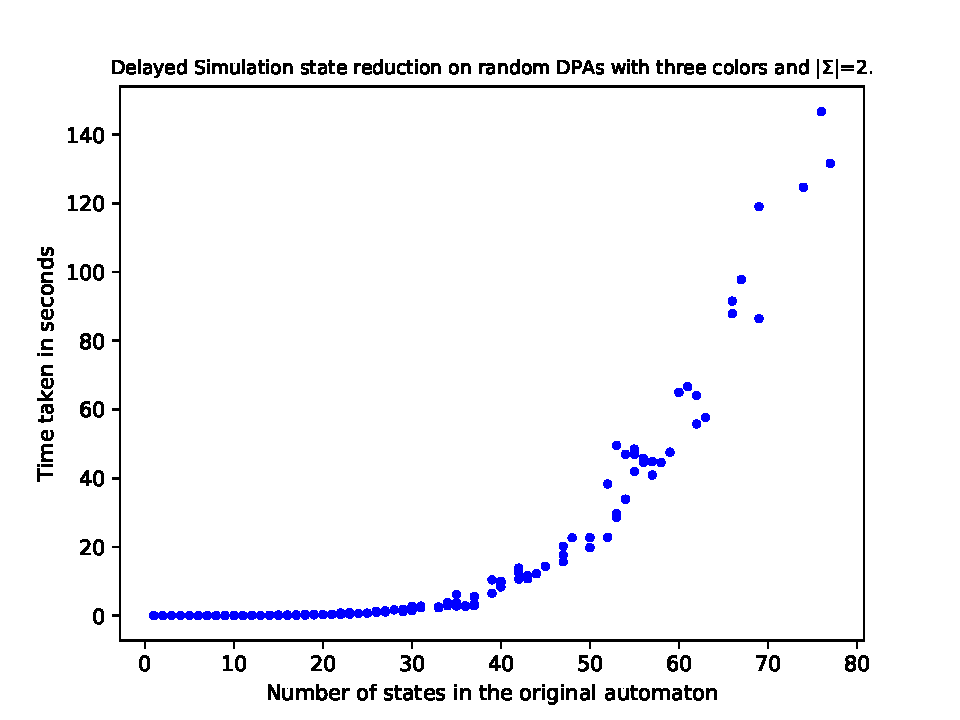
\includegraphics[page=1,height=.3\textheight]{../data/analysis/fritzwilke/gendet_ap1.pdf} 
		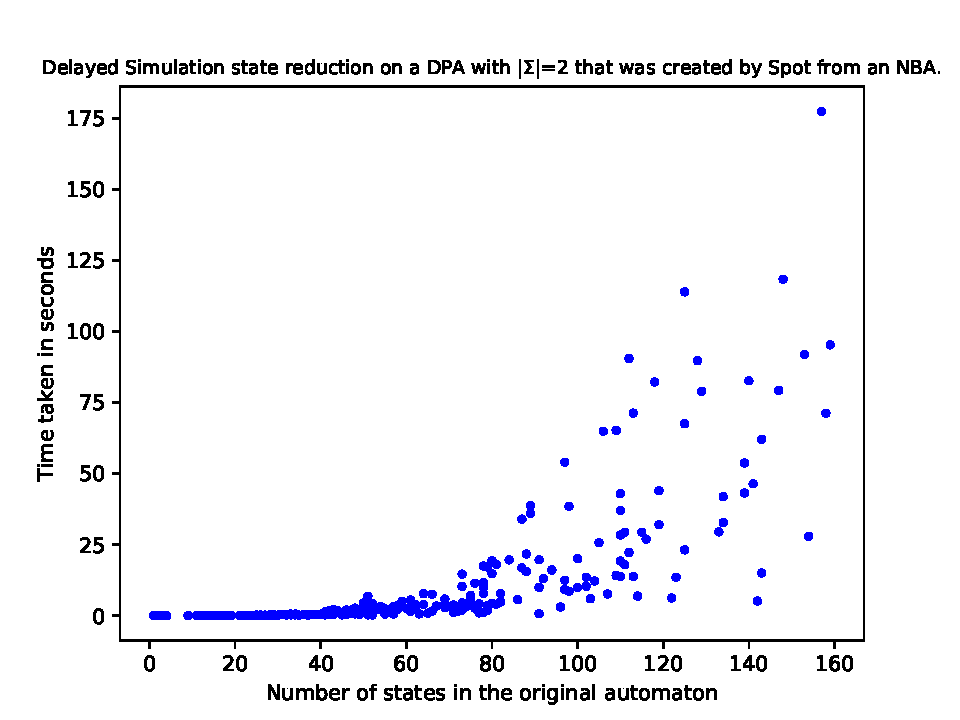
\includegraphics[page=1,height=.3\textheight]{../data/analysis/fritzwilke/detspot_ap1.pdf} 
		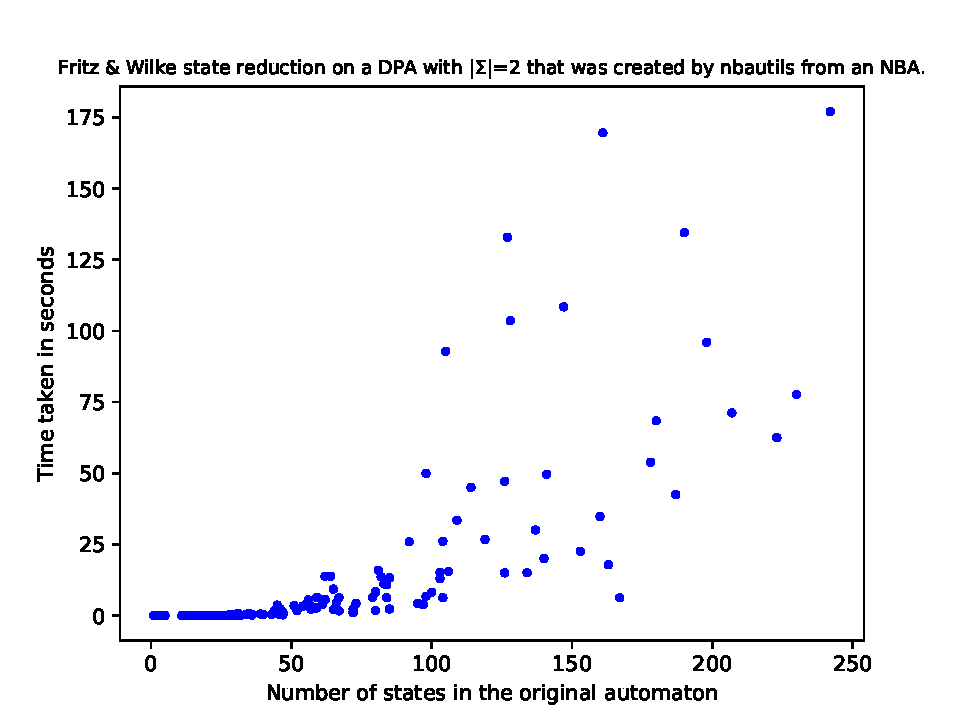
\includegraphics[page=1,height=.3\textheight]{../data/analysis/fritzwilke/detnbaut_ap1.pdf} 
		\caption{Time of the state reduction of different automata using $\mu_\text{de}$.}
		\label{fig:fritzwilke:empirical_runtime}
	\end{minipage}
\end{figure}





\section{Resetting obligations} 
In the delayed simulation automaton, \enquote{obligations} correspond to good priorities that the first state has accumulated or bad priorities that the second state has accumulated and the need for the respective other state to compensate in some way. The intuitive idea behind this concept is that an obligation that cannot be compensated, stands for an infinite run in which the acceptance differs between the two states that are being compared. The issue with the original definition is that obligations carry over, even if they can only be caused finitely often. This is demonstrated in figure \ref{fig:fritzwilke:reset_oblig_example}; the two states could be merged into one, but they are not $\equiv_\text{de}$-equivalent as can be seen in the delayed simulation automaton in figure \ref{fig:fritzwilke:reset_oblig_example_dea}.

\begin{figure}
\centering
\begin{tikzpicture}[shorten >=1pt,node distance=2cm,on grid,initial text=]
  \node[state,initial]   (0)                {0};
  \node[state]           (1) [right=of 0] {1};
  \path[->] (0) edge node [above] {a} (1)
            (1) edge [loop right] node {a} (1);
\end{tikzpicture}
\caption{Example automaton in which the states could be merged but delayed simulation separates them.}
\label{fig:fritzwilke:reset_oblig_example}
\end{figure}

\begin{figure}
\centering
\begin{tikzpicture}[shorten >=1pt,node distance=2cm,on grid,initial text=]
  \node[state]   (0)                {$0,1,0$};
  \node[state]   (1) [right=of 0] {$1,1,0$};
  \path[->] (0) edge node [above] {a} (1)
            (1) edge [loop right] node {a} (1);
\end{tikzpicture}
\caption{Delayed simulation automaton for \ref{fig:fritzwilke:reset_oblig_example}.}
\label{fig:fritzwilke:reset_oblig_example_dea}
\end{figure}

As a solution to this, we propose a simple change to the definition of the automaton which resets the obligations every time, either state moves to a new SCC. 

\begin{defn}
	Let $\mathcal{A} = (Q, \Sigma, q_0, \delta, c)$ be a DPA. We define the \emph{delayed simulation automaton with SCC resets} $\mathcal{A}_\text{deR}(p, q) = (Q_\text{de}, \Sigma, \delta_\text{deR}, F_\text{de})$ with $\delta_\text{deR}((p, q, k), a) = \delta_\text{de}((p, q, \text{reset}(p, q, k, a)), a)$. Except for the addition of the reset function, this automaton is the same as $\mathcal{A}_\text{de}$.
	
	If $p$ and $\delta(p, a)$ lie in the same SCC, as well as $q$ and $\delta(q, a)$, then we simply set $\text{reset}(p, q, k, a) =~k$. Otherwise, i.e. if any state changes its SCC, the reset comes into play and we set $\text{reset}(p, q, k, a) = \checkmark$.
	
	We write $p \leq_\text{deR} q$ if $L(\mathcal{A}_\text{deR}(p, q), q_0^\text{de}(p, q)) = \Sigma^\omega$. If also $q \leq_\text{deR} p$ holds, we write $p \equiv_\text{deR} q$.
\end{defn}

As the definition is so similar to the original delayed simulation, most results that we have already proven translate directly to the new relation. 

\begin{theorem}
	$\equiv_\text{deR}$ is a congruence relation.
\end{theorem}

\begin{lem}
\label{lem:fritzwilke:gamma_mono}
	$\gamma$ is monotonous in the third component, i.e. if $k \leq_\checkmark k'$, then $\gamma(i, j, k) \leq_\checkmark \gamma(i, j, k')$ for all $i, j \in \mathbb{N}$.
\end{lem}

\begin{proof}
	We consider each case in the definition of $\gamma$. If $i$ is odd, $i \leq_\checkmark k$ and $j \preceq_\text{p} i$, then also $i \leq_\checkmark k'$ and $\gamma(i, j, k) = \gamma(i, j, k') = \checkmark$.
	
	If $j$ is even, $j \leq_\checkmark k$ and $j \preceq_\text{p} i$, then also $j \leq_\checkmark k'$ and $\gamma(i, j, k) = \gamma(i, j, k') = \checkmark$.
	
	Otherwise, $\gamma(i, j, k) = \min \{i, j, k\}$ and $\gamma(i, j, k') = \min \{i, j, k'\}$. Since $k \leq_\checkmark k'$, $\gamma(i, j, k) \leq_\checkmark \gamma(i, j, k')$.
\end{proof}

\begin{lem}
	$\leq_\text{de} \;\subseteq\; \leq_\text{deR}$.
\end{lem}

\begin{proof} 
	Consider the two simulation automata $\mathcal{A}_\text{de}(p, q)$ and $\mathcal{A}_\text{deR}(p, q)$ and let $\alpha \in \Sigma^\omega$ be an arbitrary word. Let $(p_i, q_i, k_i)_{i \in \mathbb{N}}$ and $(p_i, q_i, l_i)_{i \in \mathbb{N}}$ be the runs of these two automata on $\alpha$. We claim that $k_i \leq_\checkmark l_i$ at every position. Then, since $L(\mathcal{A}_\text{de}(p, q), q_0^\text{de}(p, q)) = \Sigma^\omega$, both runs must be accepting.
	
	We know $k_0 = l_0$ by definition. For the sake of induction, we look at position $i+1$. If neither $p_i$ nor $q_i$ change their SCC in this step, the statement follows from Lemma \ref{lem:fritzwilke:gamma_mono}. Otherwise, $l_{i+1} = \checkmark \geq_\checkmark k_{i+1}$.
\end{proof}

\vspace{5pt}

Unfortunately, Theorem \ref{thm:fritzwilke:combine_priorities} does not translate easily to $\equiv_\text{deR}$. In fact, we were not able to find a characterization for a merger function except for the option to only merge states within single SCCs. Then, however, using the skip merger in combination with normal delayed simulation yields a result just as good.




















